% Topic 2.1: Digital Payments -- How Money Actually Moves
% Digital Finance Course - Self-contained BSC-level module
\documentclass[11pt,aspectratio=169]{beamer}
\usetheme{Madrid}

% ======================= PACKAGES =======================
\usepackage{graphicx}
\usepackage{booktabs}
\usepackage{adjustbox}
\usepackage{multicol}
\usepackage{amsmath}
\usepackage{amssymb}
\usepackage{tikz}
\usetikzlibrary{arrows,shapes,positioning,shadows,trees}
\usepackage{listings}
\usepackage{xcolor}

% ======================= COLOR DEFINITIONS =======================
% Primary color scheme: Blue/Teal for Digital Finance
\definecolor{dfblue}{RGB}{0,102,204}
\definecolor{dfteal}{RGB}{0,153,153}
\definecolor{dfcyan}{RGB}{51,187,204}
\definecolor{dflightblue}{RGB}{153,204,255}
\definecolor{dflightblue2}{RGB}{173,214,255}
\definecolor{dflightblue3}{RGB}{193,224,255}
\definecolor{dflightblue4}{RGB}{213,234,255}

% Accent colors for finance applications
\definecolor{dfgreen}{RGB}{44, 160, 44}
\definecolor{dfred}{RGB}{214, 39, 40}
\definecolor{dforange}{RGB}{255, 127, 14}
\definecolor{dfgray}{RGB}{127, 127, 127}

% Utility colors
\definecolor{lightgray}{RGB}{240, 240, 240}
\definecolor{midgray}{RGB}{180, 180, 180}
\definecolor{codebg}{RGB}{245, 245, 245}

% ======================= THEME CUSTOMIZATION =======================
% Apply Digital Finance color scheme to Madrid theme
\setbeamercolor{palette primary}{bg=dflightblue3,fg=dfblue}
\setbeamercolor{palette secondary}{bg=dflightblue2,fg=dfblue}
\setbeamercolor{palette tertiary}{bg=dfteal,fg=white}
\setbeamercolor{palette quaternary}{bg=dfblue,fg=white}

\setbeamercolor{structure}{fg=dfblue}
\setbeamercolor{section in toc}{fg=dfblue}
\setbeamercolor{subsection in toc}{fg=dfteal}
\setbeamercolor{title}{fg=dfblue}
\setbeamercolor{frametitle}{fg=dfblue,bg=dflightblue3}
\setbeamercolor{block title}{bg=dflightblue2,fg=dfblue}
\setbeamercolor{block body}{bg=dflightblue4,fg=black}

% Remove navigation symbols for cleaner look
\setbeamertemplate{navigation symbols}{}

% Clean itemize/enumerate
\setbeamertemplate{itemize items}[circle]
\setbeamertemplate{enumerate items}[default]

% Margins for readability
\setbeamersize{text margin left=8mm,text margin right=8mm}

% ======================= LISTINGS CONFIGURATION =======================
% Python code style
\lstdefinestyle{pythonstyle}{
    language=Python,
    basicstyle=\ttfamily\footnotesize,
    keywordstyle=\color{dfblue}\bfseries,
    stringstyle=\color{dforange},
    commentstyle=\color{dfgray}\itshape,
    numberstyle=\tiny\color{dfgray},
    numbers=left,
    numbersep=5pt,
    backgroundcolor=\color{codebg},
    showspaces=false,
    showstringspaces=false,
    showtabs=false,
    frame=single,
    rulecolor=\color{midgray},
    tabsize=4,
    captionpos=b,
    breaklines=true,
    breakatwhitespace=false,
    escapeinside={(*@}{@*)},
    xleftmargin=10pt,
    xrightmargin=10pt
}

% Solidity code style
\lstdefinestyle{soliditystyle}{
    language=Java, % closest approximation
    basicstyle=\ttfamily\footnotesize,
    keywordstyle=\color{dfteal}\bfseries,
    stringstyle=\color{dforange},
    commentstyle=\color{dfgray}\itshape,
    numberstyle=\tiny\color{dfgray},
    numbers=left,
    numbersep=5pt,
    backgroundcolor=\color{codebg},
    showspaces=false,
    showstringspaces=false,
    showtabs=false,
    frame=single,
    rulecolor=\color{midgray},
    tabsize=2,
    captionpos=b,
    breaklines=true,
    breakatwhitespace=false,
    escapeinside={(*@}{@*)},
    xleftmargin=10pt,
    xrightmargin=10pt,
    morekeywords={pragma, contract, function, returns, public, private, view, pure, payable, address, uint256, mapping, event, modifier}
}

% Inline code command
\newcommand{\code}[1]{\texttt{\color{dfblue}#1}}

% ======================= CUSTOM COMMANDS =======================
% Bottom annotation (Madrid-style)
\newcommand{\bottomnote}[1]{%
\vfill
\vspace{-2mm}
\textcolor{dflightblue2}{\rule{\textwidth}{0.4pt}}
\vspace{1mm}
\footnotesize
\textbf{#1}
}

% Compact list spacing
\newcommand{\compactlist}{%
\setlength{\itemsep}{0pt}%
\setlength{\parskip}{0pt}%
\setlength{\parsep}{0pt}%
}

% Chart placeholder
\newcommand{\chartplaceholder}[2][5cm]{%
\begin{center}
\begin{adjustbox}{max width=0.95\textwidth, max height=#1}
\framebox[\textwidth][c]{%
\rule{0pt}{#1}%
\textcolor{midgray}{[#2]}%
}
\end{adjustbox}
\end{center}
}

% ======================= FINANCE NOTATION MACROS =======================
% Probability and statistics
\newcommand{\E}{\mathbb{E}} % Expected value
\newcommand{\Var}{\mathrm{Var}} % Variance
\newcommand{\Cov}{\mathrm{Cov}} % Covariance
\newcommand{\Prob}{\mathbb{P}} % Probability

% Distributions
\newcommand{\Normal}{\mathcal{N}} % Normal distribution
\newcommand{\Uniform}{\mathcal{U}} % Uniform distribution

% Returns and prices
\newcommand{\Ret}{R} % Return
\newcommand{\LogRet}{r} % Log return
\newcommand{\Price}{S} % Price/Stock price
\newcommand{\Strike}{K} % Strike price

% Options and derivatives
\newcommand{\CallPrice}{C} % Call option price
\newcommand{\PutPrice}{P} % Put option price
\newcommand{\Greeks}[1]{\mathit{#1}} % Greek letters

% Risk measures
\newcommand{\VaR}{\mathrm{VaR}} % Value at Risk
\newcommand{\CVaR}{\mathrm{CVaR}} % Conditional VaR
\newcommand{\Sharpe}{\mathrm{SR}} % Sharpe Ratio

% Time series
\newcommand{\AR}{\mathrm{AR}} % Autoregressive
\newcommand{\MA}{\mathrm{MA}} % Moving average
\newcommand{\GARCH}{\mathrm{GARCH}} % GARCH

% Blockchain/Crypto
\newcommand{\Hash}{\mathrm{Hash}} % Hash function
\newcommand{\Block}{\mathcal{B}} % Block
\newcommand{\Chain}{\mathcal{C}} % Chain

% Real numbers, integers
\newcommand{\R}{\mathbb{R}}
\newcommand{\Z}{\mathbb{Z}}
\newcommand{\N}{\mathbb{N}}

% ======================= TIKZ STYLES =======================
% Styles for finance-related diagrams
\tikzstyle{process} = [rectangle, minimum width=3cm, minimum height=1cm, text centered, draw=dfblue, fill=dflightblue4, thick]
\tikzstyle{decision} = [diamond, minimum width=3cm, minimum height=1cm, text centered, draw=dfteal, fill=dflightblue4, thick]
\tikzstyle{arrow} = [thick,->,>=stealth,color=dfblue]
\tikzstyle{blockchain} = [rectangle, rounded corners, minimum width=2.5cm, minimum height=1cm, text centered, draw=dfteal, fill=dflightblue3, thick]
\tikzstyle{transaction} = [circle, minimum size=0.8cm, text centered, draw=dforange, fill=dflightblue4, thick]

% ======================= FOOTER TEMPLATE =======================
\setbeamertemplate{footline}{
    \hbox{\begin{beamercolorbox}[wd=\paperwidth,ht=2.5ex,dp=1ex,leftskip=.5em,rightskip=.5em]{author in head/foot}
    \tiny
    \textbf{Digital Finance} \hfill
    Joerg Osterrieder \hfill
    \insertdate \hfill
    Page \insertframenumber{} / \inserttotalframenumber
    \end{beamercolorbox}}
}

% ======================= SECTION DIVIDER TEMPLATE =======================
\AtBeginSection[]{
\begin{frame}[plain]
\vfill
\centering
\begin{beamercolorbox}[sep=12pt,center]{title}
\usebeamerfont{title}\LARGE\insertsection\par
\end{beamercolorbox}
\vfill
\end{frame}
}


\title{Topic 2.1: Digital Payments}
\subtitle{How Money Actually Moves}
\author{Joerg Osterrieder}
\institute{Digital Finance}
\date{2025}

\begin{document}

% ==================== SLIDE 1: TITLE ====================
\begin{frame}[plain]
\titlepage
\end{frame}

% ==================== SLIDE 2: LEARNING OBJECTIVES ====================
\begin{frame}{Learning Objectives}
\begin{block}{By the end of this topic, you will be able to:}
\begin{enumerate}
\item \textbf{Explain} the four-layer payment stack and identify each layer's function
\item \textbf{Trace} a card payment from initiation to settlement using the four-party model
\item \textbf{Compare} payment methods by speed, cost, and reversibility trade-offs
\item \textbf{Analyze} interchange economics and explain why payment fees vary
\item \textbf{Evaluate} FinTech innovations in payment infrastructure
\item \textbf{Apply} payment analysis techniques to transaction data (NB02)
\end{enumerate}
\end{block}

\vspace{3mm}
\textbf{Key Competency}: Trace a digital payment from initiation to settlement and identify where value is captured at each layer.
\end{frame}

% ==================== SLIDE 3: PREREQUISITES ====================
\begin{frame}{Prerequisites: What is a Payment?}
\begin{columns}[T]
\begin{column}{0.5\textwidth}
\textbf{Definition:}\\
A \textcolor{dfblue}{\textbf{payment}} is the transfer of value from one party (payer) to another (payee) in exchange for goods, services, or to fulfill an obligation.

\vspace{4mm}
\textbf{Three Essential Components:}
\begin{enumerate}
\item \textbf{Instruction}: Order to transfer funds
\item \textbf{Clearing}: Verification and processing
\item \textbf{Settlement}: Final, irrevocable transfer
\end{enumerate}
\end{column}
\begin{column}{0.5\textwidth}
\begin{block}{Key Terms to Know}
\begin{itemize}
\item \textbf{Payer}: Person/entity sending money
\item \textbf{Payee}: Person/entity receiving money
\item \textbf{Transaction}: A single payment event
\item \textbf{Settlement}: When funds actually move
\item \textbf{Clearing}: Reconciliation of transactions
\end{itemize}
\end{block}
\end{column}
\end{columns}

\vspace{3mm}
\textit{``Payments are the rails on which all finance travels.''}
\end{frame}

% ==================== SLIDE 4: BACKGROUND ====================
\begin{frame}{Background: Why Payments Matter}
\begin{columns}[T]
\begin{column}{0.55\textwidth}
\textbf{Payments Are Infrastructure:}
\begin{itemize}
\item Every financial transaction involves a payment
\item Global payment flows exceed \textbf{\$150 trillion annually}
\item Payment companies capture \textbf{2-3\% of all commerce}
\item Understanding payments = understanding modern finance
\end{itemize}

\vspace{3mm}
\textbf{Why FinTech Targets Payments:}
\begin{itemize}
\item Massive market size
\item Visible customer pain points
\item Technology can reduce friction
\item Network effects create moats
\end{itemize}
\end{column}
\begin{column}{0.45\textwidth}
\begin{alertblock}{The Payment Problem}
Moving money between two accounts seems simple, but involves:
\begin{itemize}
\item Multiple intermediaries
\item Complex fee structures
\item Variable settlement times
\item Security/fraud concerns
\item Regulatory compliance
\end{itemize}
\end{alertblock}
\end{column}
\end{columns}
\end{frame}

% ==================== SLIDE 5: THE PAYMENT STACK ====================
\begin{frame}{The Payment Stack: Four Layers}
\begin{center}
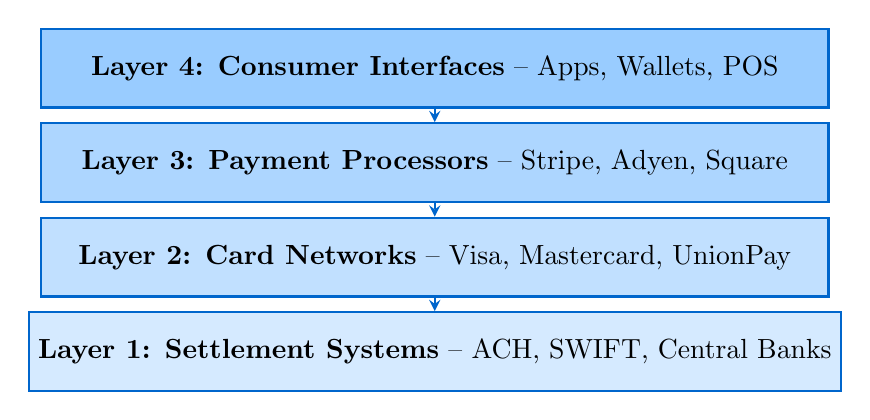
\begin{tikzpicture}[node distance=1.2cm]
% Layer boxes
\node (l4) [process, minimum width=10cm, fill=dflightblue] {\textbf{Layer 4: Consumer Interfaces} -- Apps, Wallets, POS};
\node (l3) [process, minimum width=10cm, below of=l4, fill=dflightblue2] {\textbf{Layer 3: Payment Processors} -- Stripe, Adyen, Square};
\node (l2) [process, minimum width=10cm, below of=l3, fill=dflightblue3] {\textbf{Layer 2: Card Networks} -- Visa, Mastercard, UnionPay};
\node (l1) [process, minimum width=10cm, below of=l2, fill=dflightblue4] {\textbf{Layer 1: Settlement Systems} -- ACH, SWIFT, Central Banks};

% Arrows
\draw[arrow] (l4) -- (l3);
\draw[arrow] (l3) -- (l2);
\draw[arrow] (l2) -- (l1);
\end{tikzpicture}
\end{center}

\vspace{3mm}
\begin{itemize}
\item Each layer extracts fees and adds latency
\item FinTech disruption targets specific layers
\item Understanding the stack reveals where value is captured
\end{itemize}
\end{frame}

% ==================== SLIDE 6: LAYER 1 - SETTLEMENT SYSTEMS ====================
\begin{frame}{Layer 1: Settlement Systems}
\begin{columns}[T]
\begin{column}{0.5\textwidth}
\textbf{What Settlement Systems Do:}
\begin{itemize}
\item Move actual money between banks
\item Provide finality (irreversible transfers)
\item Operated by central banks or consortia
\item Foundation of all other payment layers
\end{itemize}

\vspace{3mm}
\textbf{Key Systems:}
\begin{itemize}
\item \textbf{ACH} (US): Batch processing, 1-3 days
\item \textbf{SWIFT}: International messaging
\item \textbf{Fedwire}: Real-time US wire transfers
\item \textbf{SEPA} (EU): European transfers
\item \textbf{RTGS}: Real-time gross settlement
\end{itemize}
\end{column}
\begin{column}{0.5\textwidth}
\begin{block}{Settlement vs. Authorization}
\textbf{Authorization}: ``Yes, this payment is approved''\\
(Happens in seconds)

\vspace{2mm}
\textbf{Settlement}: ``Money has moved''\\
(Can take 1-3 days)

\vspace{2mm}
\textit{Key insight}: You can authorize instantly but settle later -- this gap creates risk and opportunity.
\end{block}
\end{column}
\end{columns}
\end{frame}

% ==================== SLIDE 7: LAYER 2 - CARD NETWORKS ====================
\begin{frame}{Layer 2: Card Networks}
\begin{columns}[T]
\begin{column}{0.5\textwidth}
\textbf{What Card Networks Do:}
\begin{itemize}
\item Connect issuing banks to acquiring banks
\item Route authorization requests
\item Set rules and standards
\item Manage fraud liability
\end{itemize}

\vspace{3mm}
\textbf{Major Networks:}
\begin{itemize}
\item \textbf{Visa}: 4B+ cards, 200+ countries
\item \textbf{Mastercard}: 2.9B+ cards globally
\item \textbf{UnionPay}: Dominant in China
\item \textbf{Amex/Discover}: Also issuers
\end{itemize}
\end{column}
\begin{column}{0.5\textwidth}
\begin{block}{Network Business Model}
\textbf{Assessment fees}: 0.13-0.15\% of each transaction

\vspace{2mm}
\textbf{Revenue sources}:
\begin{itemize}
\item Transaction fees
\item Data services
\item Value-added products
\item International currency conversion
\end{itemize}
\end{block}

\vspace{2mm}
\textbf{Visa + Mastercard} = 80\%+ of US card volume\\
\textit{Why? Network effects -- merchants accept what consumers carry.}
\end{column}
\end{columns}
\end{frame}

% ==================== SLIDE 8: LAYER 3 - PAYMENT PROCESSORS ====================
\begin{frame}{Layer 3: Payment Processors}
\begin{columns}[T]
\begin{column}{0.5\textwidth}
\textbf{What Processors Do:}
\begin{itemize}
\item Connect merchants to card networks
\item Handle technical integration
\item Manage fraud detection
\item Provide developer tools (APIs)
\end{itemize}

\vspace{3mm}
\textbf{Key Players:}
\begin{itemize}
\item \textbf{Stripe}: Developer-first, 7 lines of code
\item \textbf{Adyen}: Enterprise, single platform
\item \textbf{Square/Block}: SMB, hardware + software
\item \textbf{PayPal}: Consumer brand, two-sided
\end{itemize}
\end{column}
\begin{column}{0.5\textwidth}
\begin{block}{Processor Value Proposition}
\textbf{Before processors}:\\
Merchants negotiated directly with banks, required custom integration, complex compliance

\vspace{2mm}
\textbf{With processors}:\\
API integration in hours, bundled compliance, fraud protection, multi-network routing
\end{block}

\vspace{2mm}
\textbf{Typical markup}: 0.1-0.5\% on top of interchange
\end{column}
\end{columns}
\end{frame}

% ==================== SLIDE 9: LAYER 4 - CONSUMER INTERFACES ====================
\begin{frame}{Layer 4: Consumer Interfaces}
\begin{columns}[T]
\begin{column}{0.5\textwidth}
\textbf{What Consumer Interfaces Do:}
\begin{itemize}
\item User-facing payment experience
\item Store payment credentials securely
\item Enable convenient transactions
\item Build customer relationships
\end{itemize}

\vspace{3mm}
\textbf{Types of Interfaces:}
\begin{itemize}
\item \textbf{Mobile wallets}: Apple Pay, Google Pay
\item \textbf{P2P apps}: Venmo, Cash App, Zelle
\item \textbf{E-commerce checkout}: Shop Pay, PayPal
\item \textbf{POS terminals}: Physical card readers
\item \textbf{Bank apps}: Direct account access
\end{itemize}
\end{column}
\begin{column}{0.5\textwidth}
\begin{alertblock}{Where Competition Happens}
Layer 4 is the ``user interface'' battle:
\begin{itemize}
\item Customer owns the relationship
\item Data on spending behavior
\item Cross-sell opportunities
\item Brand differentiation
\end{itemize}

\vspace{2mm}
Most FinTech innovation targets this layer because it's closest to the customer.
\end{alertblock}
\end{column}
\end{columns}
\end{frame}

% ==================== SLIDE 10: FOUR-PARTY MODEL ====================
\begin{frame}{Card Payment Flow: The Four-Party Model}
\begin{center}
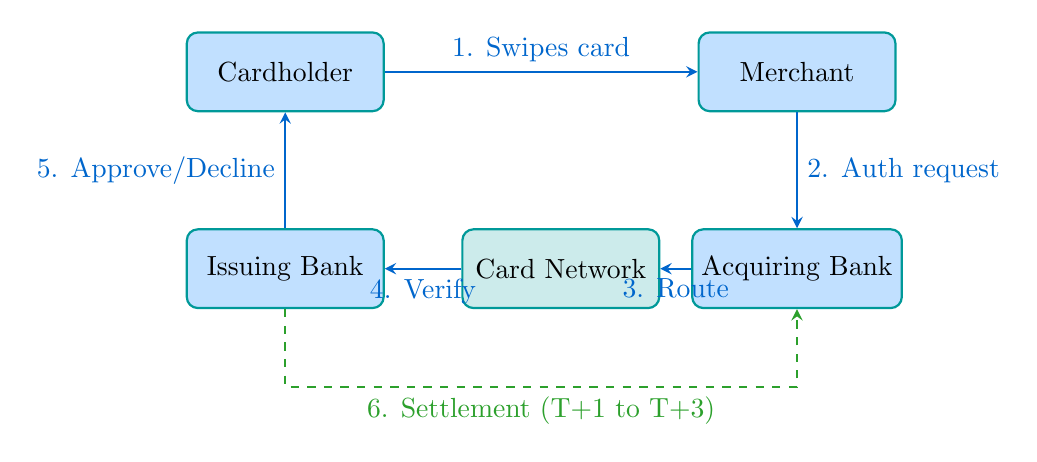
\begin{tikzpicture}[node distance=2.5cm, auto]
% Nodes
\node (cardholder) [blockchain] {Cardholder};
\node (merchant) [blockchain, right of=cardholder, xshift=4cm] {Merchant};
\node (issuer) [blockchain, below of=cardholder] {Issuing Bank};
\node (acquirer) [blockchain, below of=merchant] {Acquiring Bank};
\node (network) [blockchain, below of=cardholder, xshift=3.5cm, fill=dfteal!20] {Card Network};

% Arrows
\draw[arrow] (cardholder) -- node[above] {1. Swipes card} (merchant);
\draw[arrow] (merchant) -- node[right] {2. Auth request} (acquirer);
\draw[arrow] (acquirer) -- node[below] {3. Route} (network);
\draw[arrow] (network) -- node[below] {4. Verify} (issuer);
\draw[arrow] (issuer) -- node[left] {5. Approve/Decline} (cardholder);
\draw[arrow, dashed, color=dfgreen] (issuer) |- ++(0,-1.5) -| node[below, pos=0.25] {6. Settlement (T+1 to T+3)} (acquirer);
\end{tikzpicture}
\end{center}

\vspace{2mm}
\footnotesize
\textbf{Key insight}: Authorization is real-time ($<$2 seconds), but settlement is batch (1-3 days)
\end{frame}

% ==================== SLIDE 11: FOUR PARTIES EXPLAINED ====================
\begin{frame}{The Four Parties: Roles and Incentives}
\begin{center}
\begin{tabular}{p{2.5cm}p{4cm}p{4.5cm}}
\toprule
\textbf{Party} & \textbf{Role} & \textbf{Revenue Source} \\
\midrule
\textbf{Cardholder} & Initiates payment & (Consumer -- pays via fees/interest) \\
\textbf{Merchant} & Accepts payment & Sells goods/services \\
\textbf{Issuing Bank} & Issues card to consumer & Interchange + interest + fees \\
\textbf{Acquiring Bank} & Processes for merchant & Merchant discount rate \\
\textbf{Card Network} & Routes transactions & Assessment fees \\
\bottomrule
\end{tabular}
\end{center}

\vspace{3mm}
\begin{block}{Who Pays Whom?}
Merchant pays $\rightarrow$ Acquirer pays $\rightarrow$ Network pays $\rightarrow$ Issuer\\
The \textbf{issuing bank} receives the largest share (interchange) because they bear the credit/fraud risk.
\end{block}
\end{frame}

% ==================== SLIDE 12: INTERCHANGE ECONOMICS ====================
\begin{frame}{Interchange Economics: Who Pays What}
\begin{columns}[T]
\begin{column}{0.55\textwidth}
\textbf{Fee Breakdown (Typical US Card Transaction):}
\begin{itemize}
\item \textbf{Interchange}: 1.5-2.5\% $\rightarrow$ Issuing bank
\item \textbf{Assessment}: 0.13-0.15\% $\rightarrow$ Card network
\item \textbf{Processor markup}: 0.1-0.5\% $\rightarrow$ Payment processor
\end{itemize}

\vspace{3mm}
\textbf{Total: 2.0-3.5\%} of transaction value
\end{column}
\begin{column}{0.45\textwidth}
\begin{block}{Why So Expensive?}
\begin{itemize}
\item Fraud liability shift
\item Reward program funding
\item Network effects protection
\item Regulatory capture
\end{itemize}
\end{block}
\end{column}
\end{columns}

\vspace{3mm}
\begin{alertblock}{EU vs US Comparison}
EU interchange capped at 0.2\% (debit) / 0.3\% (credit) by regulation.\\
US averages 2.2\% -- \textbf{10x higher}. Why the difference? Regulation.
\end{alertblock}
\end{frame}

% ==================== SLIDE 13: INTERCHANGE CALCULATION ====================
\begin{frame}{Understanding Interchange: A Worked Example}
\begin{block}{Scenario: \$100 Purchase at a Retail Store}
\end{block}

\begin{columns}[T]
\begin{column}{0.5\textwidth}
\textbf{Fee Calculation:}
\begin{itemize}
\item Interchange (1.8\%): \$1.80
\item Assessment (0.14\%): \$0.14
\item Processor (0.3\% + \$0.10): \$0.40
\end{itemize}

\vspace{2mm}
\textbf{Total fees}: \$2.34\\
\textbf{Merchant receives}: \$97.66
\end{column}
\begin{column}{0.5\textwidth}
\textbf{Fee Distribution:}
\begin{itemize}
\item Issuing bank: \$1.80 (77\%)
\item Card network: \$0.14 (6\%)
\item Processor: \$0.40 (17\%)
\end{itemize}

\vspace{2mm}
\textit{The issuing bank captures most value because they:}
\begin{itemize}
\item Bear credit risk
\item Fund rewards
\item Handle disputes
\end{itemize}
\end{column}
\end{columns}

\vspace{3mm}
\textbf{Key insight}: On a 3\% retail margin, payment fees can consume 70\%+ of profit
\end{frame}

% ==================== SLIDE 14: PAYMENT METHODS COMPARISON ====================
\begin{frame}{Payment Methods: Speed vs Cost Matrix}
\begin{center}
\begin{tabular}{lccc}
\toprule
\textbf{Method} & \textbf{Settlement} & \textbf{Cost} & \textbf{Reversibility} \\
\midrule
Wire Transfer (SWIFT) & 1-5 days & \$15-50 flat & Difficult \\
ACH (US) & 1-3 days & \$0.20-1.50 & Reversible (60 days) \\
Card (Visa/MC) & 1-3 days & 2-3\% & Chargeback rights \\
SEPA (EU) & Same day & $<$\euro 0.20 & Limited \\
Real-Time (FedNow/PIX) & Seconds & \$0.01-0.05 & Final \\
Crypto (Bitcoin) & 10-60 min & Variable & Final \\
Stablecoins & Seconds-minutes & \$0.01-5 & Final \\
\bottomrule
\end{tabular}
\end{center}

\vspace{3mm}
\textbf{Key tradeoff}: Speed and finality vs. consumer protection (reversibility)
\end{frame}

% ==================== SLIDE 15: WIRE TRANSFERS ====================
\begin{frame}{Wire Transfers: The Premium Option}
\begin{columns}[T]
\begin{column}{0.5\textwidth}
\textbf{What is a Wire Transfer?}
\begin{itemize}
\item Direct bank-to-bank transfer
\item Uses SWIFT network internationally
\item Fedwire for domestic US
\item High certainty of payment
\end{itemize}

\vspace{3mm}
\textbf{Characteristics:}
\begin{itemize}
\item \textbf{Speed}: 1-3 days (domestic), 3-5 (international)
\item \textbf{Cost}: \$25-50 flat fee
\item \textbf{Use case}: Large transactions, real estate
\end{itemize}
\end{column}
\begin{column}{0.5\textwidth}
\begin{block}{Why So Expensive?}
Wire transfer fees cover:
\begin{itemize}
\item Manual processing by bank staff
\item AML/KYC compliance checks
\item SWIFT network messaging fees
\item Correspondent bank fees
\item Guaranteed settlement
\end{itemize}
\end{block}

\vspace{2mm}
\textbf{Key insight}: Wire transfers are not cost-effective at any transaction size compared to ACH, but offer certainty.
\end{column}
\end{columns}
\end{frame}

% ==================== SLIDE 16: ACH PAYMENTS ====================
\begin{frame}{ACH: The Workhorse of US Payments}
\begin{columns}[T]
\begin{column}{0.5\textwidth}
\textbf{What is ACH?}
\begin{itemize}
\item Automated Clearing House
\item Batch processing system
\item Run by Nacha (formerly NACHA)
\item Handles 30B+ transactions/year
\end{itemize}

\vspace{3mm}
\textbf{Characteristics:}
\begin{itemize}
\item \textbf{Speed}: 1-3 business days
\item \textbf{Cost}: \$0.20-1.50 per transaction
\item \textbf{Fee structure}: 0.1\% + \$0.50 typical
\end{itemize}
\end{column}
\begin{column}{0.5\textwidth}
\begin{block}{Common ACH Uses}
\begin{itemize}
\item Payroll direct deposit
\item Bill payments
\item Government benefits
\item Subscription payments
\item Bank-to-bank transfers
\end{itemize}
\end{block}

\vspace{2mm}
\begin{alertblock}{Best For}
Small to medium transactions under \$5,000 where speed is not critical. Most cost-effective payment method for recurring payments.
\end{alertblock}
\end{column}
\end{columns}
\end{frame}

% ==================== SLIDE 17: DIGITAL WALLETS ====================
\begin{frame}{Digital Wallets: Speed vs. Cost}
\begin{columns}[T]
\begin{column}{0.5\textwidth}
\textbf{What are Digital Wallets?}
\begin{itemize}
\item Services like PayPal, Venmo, Cash App
\item Store payment credentials
\item Enable instant transfers
\item Often include social features
\end{itemize}

\vspace{3mm}
\textbf{Characteristics:}
\begin{itemize}
\item \textbf{Speed}: Instant (within network)
\item \textbf{Cost}: 2.9\% + \$0.30 (merchant)
\item \textbf{P2P}: Often free within network
\end{itemize}
\end{column}
\begin{column}{0.5\textwidth}
\begin{block}{Why Higher Fees?}
Digital wallet premium covers:
\begin{itemize}
\item Instant settlement
\item Fraud protection
\item Dispute resolution
\item Platform maintenance
\item Customer support
\end{itemize}
\end{block}

\vspace{2mm}
\textbf{Trade-off}: Highest percentage fee (2.9\%) but fastest settlement and best user experience.
\end{column}
\end{columns}
\end{frame}

% ==================== SLIDE 18: REAL-TIME PAYMENT SYSTEMS ====================
\begin{frame}{Real-Time Payment Systems: Global Adoption}
\begin{columns}[T]
\begin{column}{0.5\textwidth}
\textbf{Live Systems (2024):}
\begin{itemize}
\item \textbf{PIX (Brazil)}: 150M+ users, 3B+ txns/month
\item \textbf{UPI (India)}: 300M+ users, 10B+ txns/month
\item \textbf{FPS (UK)}: 4B+ txns/year
\item \textbf{FedNow (US)}: Launched 2023
\item \textbf{TIPS (EU)}: Euro-wide instant
\end{itemize}
\end{column}
\begin{column}{0.5\textwidth}
\begin{block}{Impact on FinTech}
\begin{itemize}
\item Commoditizes payment rails
\item Threatens card networks
\item Enables new business models
\item Government as infrastructure provider
\end{itemize}
\end{block}
\end{column}
\end{columns}

\vspace{3mm}
\begin{alertblock}{Strategic Question}
If real-time payments are nearly free, where does payment FinTech capture value?
\end{alertblock}
\end{frame}

% ==================== SLIDE 19: CROSS-BORDER PAYMENTS ====================
\begin{frame}{Cross-Border Payments: The \$150 Trillion Opportunity}
\begin{center}
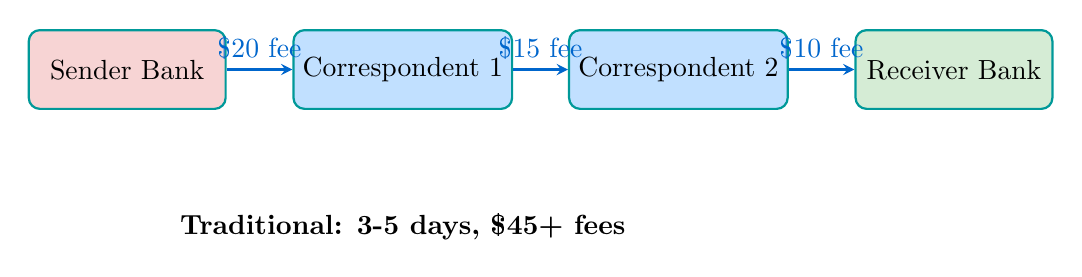
\begin{tikzpicture}[node distance=1.5cm]
% Traditional path
\node (sender) [blockchain, fill=dfred!20] {Sender Bank};
\node (corr1) [blockchain, right of=sender, xshift=2cm] {Correspondent 1};
\node (corr2) [blockchain, right of=corr1, xshift=2cm] {Correspondent 2};
\node (receiver) [blockchain, right of=corr2, xshift=2cm, fill=dfgreen!20] {Receiver Bank};

\draw[arrow] (sender) -- node[above] {\$20 fee} (corr1);
\draw[arrow] (corr1) -- node[above] {\$15 fee} (corr2);
\draw[arrow] (corr2) -- node[above] {\$10 fee} (receiver);

% Labels
\node[below of=corr1, yshift=-0.5cm] {\textbf{Traditional: 3-5 days, \$45+ fees}};
\end{tikzpicture}
\end{center}

\vspace{5mm}
\textbf{FinTech Solutions:}
\begin{columns}[T]
\begin{column}{0.33\textwidth}
\textbf{Wise (TransferWise)}\\
Peer-matching + local rails\\
\textcolor{dfgreen}{70\% cheaper}
\end{column}
\begin{column}{0.33\textwidth}
\textbf{Ripple/XRP}\\
Blockchain settlement\\
\textcolor{dfgreen}{Seconds, not days}
\end{column}
\begin{column}{0.33\textwidth}
\textbf{Stablecoin Rails}\\
USDC on-chain transfers\\
\textcolor{dfgreen}{24/7 settlement}
\end{column}
\end{columns}
\end{frame}

% ==================== SLIDE 20: PAYMENT FAILURES ====================
\begin{frame}{Payment Failures: Understanding the Funnel}
\begin{columns}[T]
\begin{column}{0.5\textwidth}
\textbf{Where Payments Fail:}
\begin{enumerate}
\item \textbf{Insufficient funds}: 30-40\%
\item \textbf{Fraud blocks}: 20-25\%
\item \textbf{Network timeouts}: 10-15\%
\item \textbf{Card expired}: 10-15\%
\item \textbf{3DS abandonment}: 10-15\%
\item \textbf{Other}: 5-10\%
\end{enumerate}
\end{column}
\begin{column}{0.5\textwidth}
\begin{block}{Business Impact}
\begin{itemize}
\item Average decline rate: \textbf{15-20\%}
\item Each 1\% improvement = significant revenue
\item ``False positives'' (good txns blocked) cost more than fraud
\end{itemize}
\end{block}
\end{column}
\end{columns}

\vspace{3mm}
\begin{alertblock}{Transaction Status Distribution}
Realistic payment systems: 92\% completed, 5\% pending, 3\% failed.\\
Understanding failure rates is critical for revenue projections and customer experience.
\end{alertblock}
\end{frame}

% ==================== SLIDE 21: SETTLEMENT TIME ANALYSIS ====================
\begin{frame}{Settlement Time: Why Percentiles Matter}
\begin{columns}[T]
\begin{column}{0.5\textwidth}
\textbf{What is Settlement Time?}\\
The period between payment initiation and when funds are actually, irrevocably available to the recipient.

\vspace{3mm}
\textbf{Why Analyze Percentiles?}
\begin{itemize}
\item \textbf{P50 (median)}: Typical experience
\item \textbf{P90-P95}: What ``most'' experience
\item \textbf{P99}: Worst-case scenarios
\end{itemize}
\end{column}
\begin{column}{0.5\textwidth}
\begin{block}{Business Applications}
\textbf{SLA Design}:\\
``95\% of ACH payments settle within 3 days''

\vspace{2mm}
\textbf{Liquidity Planning}:\\
Know when funds will be available

\vspace{2mm}
\textbf{Customer Expectations}:\\
Set accurate delivery promises

\vspace{2mm}
\textbf{Outlier Detection}:\\
Identify transactions needing investigation
\end{block}
\end{column}
\end{columns}
\end{frame}

% ==================== SLIDE 22: FINTECH PAYMENT INNOVATORS ====================
\begin{frame}{FinTech Payment Innovators: Business Model Analysis}
\begin{center}
\begin{tabular}{p{2.5cm}p{3.5cm}p{4.5cm}}
\toprule
\textbf{Company} & \textbf{Innovation} & \textbf{Revenue Model} \\
\midrule
\textbf{Stripe} & Developer-first APIs, embedded finance & 2.9\% + \$0.30 per txn \\
\textbf{Square/Block} & Hardware + software bundle, SMB focus & 2.6\% + \$0.10 per txn \\
\textbf{Adyen} & Single platform, enterprise & Interchange++ (transparent) \\
\textbf{PayPal} & Two-sided network, checkout & 3.49\% + \$0.49 per txn \\
\textbf{Wise} & Mid-market FX, transparency & 0.5-2\% of transfer \\
\textbf{Plaid} & Account connectivity & Per-API-call pricing \\
\bottomrule
\end{tabular}
\end{center}

\vspace{2mm}
\textbf{Key insight}: Most FinTechs are \textit{layers on top of} traditional rails, not replacements
\end{frame}

% ==================== SLIDE 23: BNPL ====================
\begin{frame}{Buy Now Pay Later (BNPL): Disrupting Card Credit}
\begin{columns}[T]
\begin{column}{0.5\textwidth}
\textbf{How BNPL Works:}
\begin{enumerate}
\item Consumer selects BNPL at checkout
\item BNPL provider pays merchant (minus fee)
\item Consumer repays in 4 installments
\item No interest (if on-time)
\end{enumerate}

\vspace{3mm}
\textbf{Key Players:}
Klarna, Affirm, Afterpay, PayPal Pay in 4
\end{column}
\begin{column}{0.5\textwidth}
\begin{block}{Revenue Sources}
\begin{itemize}
\item Merchant fees: 4-8\% (higher than cards!)
\item Late fees: \$7-10 per missed payment
\item Interest on longer-term loans
\end{itemize}
\end{block}

\begin{alertblock}{Risks}
\begin{itemize}
\item Credit losses (no traditional underwriting)
\item Regulatory scrutiny increasing
\item Consumer debt concerns
\end{itemize}
\end{alertblock}
\end{column}
\end{columns}
\end{frame}

% ==================== SLIDE 24: PAYMENT NETWORK ANALYSIS ====================
\begin{frame}{Payment Network Analysis: Graph Perspectives}
\begin{columns}[T]
\begin{column}{0.5\textwidth}
\textbf{Why Visualize Payment Networks?}
\begin{itemize}
\item Identify key hubs (major players)
\item Detect fraud patterns
\item Understand money flow
\item Assess systemic risks
\end{itemize}

\vspace{3mm}
\textbf{Network Metrics:}
\begin{itemize}
\item \textbf{Degree centrality}: Number of connections
\item \textbf{Betweenness}: Bridge between groups
\item \textbf{PageRank}: Importance by connections
\item \textbf{Net flow}: Sender vs. receiver
\end{itemize}
\end{column}
\begin{column}{0.5\textwidth}
\begin{block}{Centrality Explained}
\textbf{Degree}: How many parties you transact with\\
\textit{High = very active}

\vspace{2mm}
\textbf{Betweenness}: How often you're on paths between others\\
\textit{High = critical bridge/bottleneck}

\vspace{2mm}
\textbf{PageRank}: Importance based on who connects to you\\
\textit{High = trusted/influential}
\end{block}
\end{column}
\end{columns}
\end{frame}

% ==================== SLIDE 25: HANDS-ON EXERCISE INTRO ====================
\begin{frame}{Hands-On Exercise: NB02 Payment Transaction Analysis}
\begin{block}{Notebook Overview}
Analyze simulated payment transaction data to understand:
\begin{itemize}
\item Payment method characteristics and trade-offs
\item Fee structures and cost optimization
\item Settlement time distributions
\item Network analysis and fraud detection concepts
\end{itemize}
\end{block}

\vspace{3mm}
\textbf{Six Payment Methods Analyzed:}
\begin{enumerate}
\item \textbf{Wire Transfer}: High fixed fees, 1-3 days
\item \textbf{ACH}: Low cost, batch processing
\item \textbf{Credit Card}: Instant authorization, 2.5\% + \$0.30
\item \textbf{Debit Card}: Direct account access, 1.5\%
\item \textbf{Digital Wallet}: Instant, 2.9\% + \$0.30
\item \textbf{Cryptocurrency}: Variable, blockchain-based
\end{enumerate}
\end{frame}

% ==================== SLIDE 26: HANDS-ON EXERCISE TASKS ====================
\begin{frame}{NB02 Exercise Tasks}
\begin{columns}[T]
\begin{column}{0.5\textwidth}
\textbf{Part 1: Data Exploration}
\begin{itemize}
\item Load and examine transaction dataset
\item Analyze transaction amount distributions
\item Explore temporal patterns (business hours bias)
\item Calculate summary statistics
\end{itemize}

\vspace{3mm}
\textbf{Part 2: Fee Analysis}
\begin{itemize}
\item Compare fee structures across methods
\item Calculate effective fee rates
\item Find optimal method by transaction size
\item Visualize cost curves
\end{itemize}
\end{column}
\begin{column}{0.5\textwidth}
\textbf{Part 3: Settlement Analysis}
\begin{itemize}
\item Calculate percentile distributions
\item Design SLA thresholds
\item Identify outliers for investigation
\end{itemize}

\vspace{3mm}
\textbf{Part 4: Network Analysis}
\begin{itemize}
\item Build payment network graph
\item Calculate centrality metrics
\item Identify hubs and bridges
\item Analyze net flows
\end{itemize}

\vspace{3mm}
\begin{alertblock}{Key Skills}
Data manipulation, visualization, network graphs, business intelligence
\end{alertblock}
\end{column}
\end{columns}
\end{frame}

% ==================== SLIDE 27: DISCUSSION - PAYMENT CHOICE ====================
\begin{frame}{Discussion: Choosing the Right Payment Method}
\begin{block}{Scenario Analysis}
For each scenario, which payment method would you recommend and why?
\end{block}

\begin{columns}[T]
\begin{column}{0.5\textwidth}
\textbf{1. Monthly rent payment (\$2,000)}
\begin{itemize}
\item Speed not critical
\item Recurring
\item Cost-sensitive
\end{itemize}
\textcolor{dfgreen}{\textit{Answer: ACH (lowest cost)}}

\vspace{3mm}
\textbf{2. Coffee shop purchase (\$5)}
\begin{itemize}
\item Convenience key
\item High volume, low value
\item Customer experience matters
\end{itemize}
\textcolor{dfgreen}{\textit{Answer: Card/Wallet (speed + UX)}}
\end{column}
\begin{column}{0.5\textwidth}
\textbf{3. Real estate closing (\$500,000)}
\begin{itemize}
\item Certainty required
\item Large value
\item Legal requirements
\end{itemize}
\textcolor{dfgreen}{\textit{Answer: Wire transfer (guaranteed)}}

\vspace{3mm}
\textbf{4. International supplier payment}
\begin{itemize}
\item Cross-border
\item FX exposure
\item Speed vs. cost trade-off
\end{itemize}
\textcolor{dfgreen}{\textit{Answer: Wise or stablecoin (cost + speed)}}
\end{column}
\end{columns}
\end{frame}

% ==================== SLIDE 28: DISCUSSION - FINTECH DISRUPTION ====================
\begin{frame}{Discussion: Where Will FinTech Disrupt Payments?}
\begin{columns}[T]
\begin{column}{0.5\textwidth}
\textbf{Most Vulnerable to Disruption:}
\begin{itemize}
\item \textbf{Cross-border}: High fees, slow speed
\item \textbf{B2B payments}: Still paper-based
\item \textbf{Interchange}: Regulatory pressure
\item \textbf{Real-time settlement}: Government competition
\end{itemize}

\vspace{3mm}
\textbf{Hardest to Disrupt:}
\begin{itemize}
\item Card networks (network effects)
\item Settlement systems (regulatory capture)
\item Consumer habits (trust, convenience)
\end{itemize}
\end{column}
\begin{column}{0.5\textwidth}
\begin{alertblock}{Discussion Questions}
\begin{enumerate}
\item If FedNow makes instant payments free, what happens to Visa?
\item Why haven't cryptocurrencies replaced traditional payments?
\item What would it take to displace card networks?
\item Is BNPL sustainable or venture-subsidized?
\end{enumerate}
\end{alertblock}
\end{column}
\end{columns}
\end{frame}

% ==================== SLIDE 29: DISCUSSION - PAYMENT VOLUME ANALYSIS ====================
\begin{frame}{Application: Payment Volume Business Intelligence}
\begin{block}{Four Key Uses of Payment Volume Analysis}
\end{block}

\begin{columns}[T]
\begin{column}{0.5\textwidth}
\textbf{1. Capacity Planning}
\begin{itemize}
\item Predict peak load times
\item Size infrastructure
\item Plan staffing for support
\end{itemize}

\vspace{3mm}
\textbf{2. Fraud Detection}
\begin{itemize}
\item Unusual hour transactions
\item Abnormal volume spikes
\item Network pattern anomalies
\end{itemize}
\end{column}
\begin{column}{0.5\textwidth}
\textbf{3. Business Intelligence}
\begin{itemize}
\item Customer behavior patterns
\item Seasonal trends
\item Product category analysis
\end{itemize}

\vspace{3mm}
\textbf{4. Revenue Forecasting}
\begin{itemize}
\item Fee income projections
\item Transaction mix shifts
\item Growth rate modeling
\end{itemize}
\end{column}
\end{columns}

\vspace{3mm}
\textbf{Key insight}: Transaction count vs. volume tell different stories -- a method can have many small transactions or few large ones.
\end{frame}

% ==================== SLIDE 30: APPLICATION - REAL-WORLD ====================
\begin{frame}{Real-World Applications}
\begin{columns}[T]
\begin{column}{0.33\textwidth}
\textbf{Fraud Detection}
\begin{itemize}
\item Unusual network patterns
\item Velocity checks
\item Geographic anomalies
\item Behavioral biometrics
\end{itemize}

\vspace{2mm}
\textit{Payment data reveals fraud rings through clustering.}
\end{column}
\begin{column}{0.33\textwidth}
\textbf{Liquidity Management}
\begin{itemize}
\item Settlement time prediction
\item Cash flow forecasting
\item Working capital optimization
\item Float management
\end{itemize}

\vspace{2mm}
\textit{Know when funds will be available.}
\end{column}
\begin{column}{0.33\textwidth}
\textbf{Cost Optimization}
\begin{itemize}
\item Method selection by size
\item Routing optimization
\item Fee negotiation data
\item Processor comparison
\end{itemize}

\vspace{2mm}
\textit{Right method for each transaction.}
\end{column}
\end{columns}

\vspace{5mm}
\begin{block}{Career Application}
Payment analysts at FinTechs, banks, and merchants use these techniques daily to optimize billions in transaction flow.
\end{block}
\end{frame}

% ==================== SLIDE 31: EXECUTIVE SUMMARY ====================
\begin{frame}{Executive Summary: Key Takeaways}
\begin{enumerate}
\item \textbf{Payments are multi-layered}: Consumer interfaces $\rightarrow$ processors $\rightarrow$ networks $\rightarrow$ settlement systems. Each layer extracts value.

\item \textbf{Speed vs. protection tradeoff}: Faster payments = less reversibility. Real-time is convenient but risky for consumers.

\item \textbf{Interchange is the prize}: Issuing banks capture 1.5-2.5\% on every card transaction. This funds rewards and creates massive industry.

\item \textbf{Real-time rails are commoditizing}: Government systems like PIX, UPI, FedNow threaten card network dominance.

\item \textbf{Most FinTechs are layers, not replacements}: Stripe, PayPal, Square build on top of existing rails rather than replacing them.
\end{enumerate}

\vspace{3mm}
\begin{block}{One Sentence Summary}
Digital payments flow through a four-layer stack where each layer captures fees, and understanding this architecture reveals both where value is extracted and where FinTech disruption is possible.
\end{block}
\end{frame}

% ==================== SLIDE 32: CONCEPT MAP ====================
\begin{frame}{Concept Map: Digital Payments Ecosystem}
\begin{center}
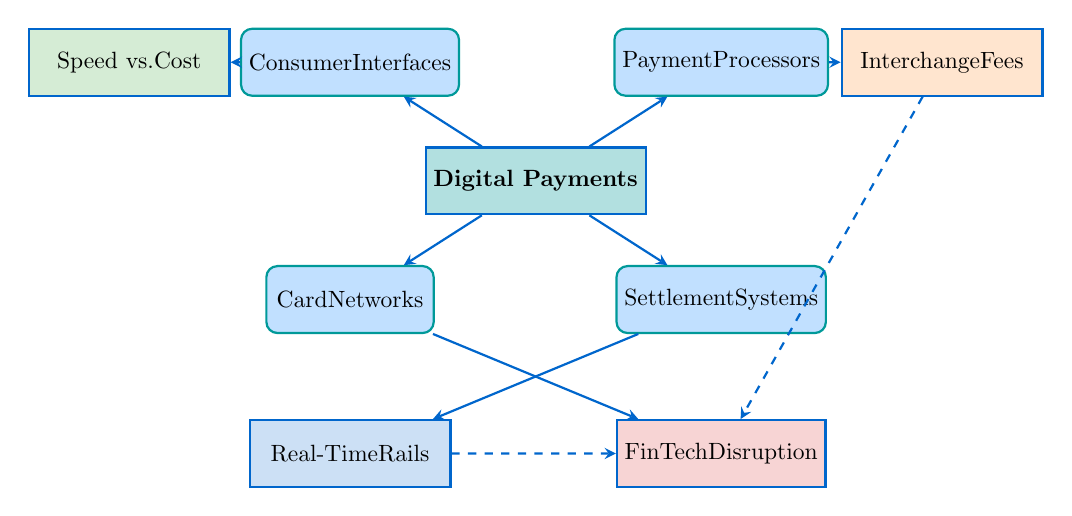
\begin{tikzpicture}[node distance=1.8cm, scale=0.85, transform shape]
% Central node
\node (payments) [process, fill=dfteal!30, minimum width=3cm] {\textbf{Digital Payments}};

% Layer nodes
\node (consumer) [blockchain, above left of=payments, xshift=-1.5cm, yshift=0.5cm] {Consumer\\Interfaces};
\node (processor) [blockchain, above right of=payments, xshift=1.5cm, yshift=0.5cm] {Payment\\Processors};
\node (network) [blockchain, below left of=payments, xshift=-1.5cm, yshift=-0.5cm] {Card\\Networks};
\node (settlement) [blockchain, below right of=payments, xshift=1.5cm, yshift=-0.5cm] {Settlement\\Systems};

% Concept nodes
\node (fee) [process, right of=processor, xshift=1.5cm, fill=dforange!20] {Interchange\\Fees};
\node (speed) [process, left of=consumer, xshift=-1.5cm, fill=dfgreen!20] {Speed vs.\\Cost};
\node (fintech) [process, below of=settlement, yshift=-0.5cm, fill=dfred!20] {FinTech\\Disruption};
\node (realtime) [process, below of=network, yshift=-0.5cm, fill=dfblue!20] {Real-Time\\Rails};

% Arrows
\draw[arrow] (payments) -- (consumer);
\draw[arrow] (payments) -- (processor);
\draw[arrow] (payments) -- (network);
\draw[arrow] (payments) -- (settlement);
\draw[arrow] (processor) -- (fee);
\draw[arrow] (consumer) -- (speed);
\draw[arrow] (settlement) -- (realtime);
\draw[arrow] (network) -- (fintech);
\draw[arrow, dashed] (realtime) -- (fintech);
\draw[arrow, dashed] (fee) -- (fintech);
\end{tikzpicture}
\end{center}
\end{frame}

% ==================== SLIDE 33: KEY TERMS 1 ====================
\begin{frame}{Key Terms \& Definitions (Part 1)}
\begin{description}
\item[\textcolor{dfblue}{Settlement}] The final, irrevocable transfer of funds from payer to payee. Distinct from authorization.

\item[\textcolor{dfblue}{Interchange}] The fee paid by the acquiring bank to the issuing bank for each card transaction. Typically 1.5-2.5\% in the US.

\item[\textcolor{dfblue}{Four-Party Model}] Card payment structure involving cardholder, merchant, issuing bank, and acquiring bank, connected by the card network.

\item[\textcolor{dfblue}{ACH}] Automated Clearing House -- US batch payment system for low-cost, non-urgent transfers. Settlement in 1-3 days.

\item[\textcolor{dfblue}{SWIFT}] Society for Worldwide Interbank Financial Telecommunication -- messaging network for international wire transfers.
\end{description}
\end{frame}

% ==================== SLIDE 34: KEY TERMS 2 ====================
\begin{frame}{Key Terms \& Definitions (Part 2)}
\begin{description}
\item[\textcolor{dfblue}{Payment Processor}] Company that handles technical integration between merchants and card networks (e.g., Stripe, Adyen).

\item[\textcolor{dfblue}{Merchant Discount Rate (MDR)}] Total fee paid by merchant for accepting card payments, including interchange + assessment + processor markup.

\item[\textcolor{dfblue}{Real-Time Payments}] Systems enabling instant, irrevocable fund transfers (e.g., PIX, UPI, FedNow).

\item[\textcolor{dfblue}{BNPL (Buy Now Pay Later)}] Payment method allowing consumers to split purchases into installments, typically 4 payments over 6 weeks.

\item[\textcolor{dfblue}{Chargeback}] Consumer's right to dispute and reverse a card transaction, typically within 60-120 days.
\end{description}
\end{frame}

% ==================== SLIDE 35: COMMON MISCONCEPTIONS ====================
\begin{frame}{Common Misconceptions: Myth vs. Reality}
\begin{columns}[T]
\begin{column}{0.5\textwidth}
\textbf{Myth 1:} ``Card payments are instant''\\
\textcolor{dfred}{Reality:} Authorization is instant, but settlement takes 1-3 days. Merchants don't receive funds immediately.

\vspace{4mm}
\textbf{Myth 2:} ``Wire transfers are always best for large amounts''\\
\textcolor{dfred}{Reality:} Wire transfers are never the most cost-effective option due to high fixed fees. ACH is cheaper even for large amounts. Wire transfers are used for certainty, not cost.
\end{column}
\begin{column}{0.5\textwidth}
\textbf{Myth 3:} ``FinTechs have replaced traditional payment rails''\\
\textcolor{dfred}{Reality:} Most FinTechs (Stripe, PayPal, Square) are layers \textit{on top of} existing infrastructure, not replacements.

\vspace{4mm}
\textbf{Myth 4:} ``Lower fees always mean better payment method''\\
\textcolor{dfred}{Reality:} Speed, reversibility, and consumer protection matter. Faster, irreversible payments (crypto, real-time) trade consumer protection for efficiency.
\end{column}
\end{columns}
\end{frame}

% ==================== SLIDE 36: SELF-ASSESSMENT Q1 ====================
\begin{frame}{Self-Assessment Question 1}
\begin{block}{Question}
What are the six payment methods analyzed in the NB02 Payment Analysis notebook?
\end{block}

\vspace{3mm}
\textbf{Options:}
\begin{enumerate}[A.]
\item Wire Transfer, ACH, SEPA, Check, Cash, Bitcoin
\item Wire Transfer, ACH, Credit Card, Debit Card, Digital Wallet, Cryptocurrency
\item SWIFT, FedWire, PayPal, Venmo, Cash App, Stripe
\item RTGS, DNS, Credit Card, Prepaid Card, Money Order, Check
\end{enumerate}

\vspace{5mm}
\pause
\textcolor{dfgreen}{\textbf{Answer: B}}\\
The notebook analyzes six payment methods: Wire Transfer, ACH, Credit Card, Debit Card, Digital Wallet, and Cryptocurrency. Each has distinct characteristics in terms of speed, cost, and settlement time.
\end{frame}

% ==================== SLIDE 37: SELF-ASSESSMENT Q2-3 ====================
\begin{frame}{Self-Assessment Questions 2-3}
\begin{block}{Question 2: Network Analysis}
In network analysis, what does `degree centrality' measure in a payment network?
\end{block}
\textbf{Answer:} The number of direct connections (other parties) a node has in the network. High degree centrality indicates a party is highly active -- essentially counting how many other parties a given party transacts with.

\vspace{5mm}
\begin{block}{Question 3: Business Intelligence}
What does the notebook identify as the four key business intelligence uses of payment volume analysis?
\end{block}
\textbf{Answer:} \textbf{Capacity Planning} (system load), \textbf{Fraud Detection} (unusual patterns), \textbf{Business Intelligence} (customer behavior), and \textbf{Revenue Forecasting} (fee income prediction). These insights drive operational and strategic decisions.
\end{frame}

% ==================== SLIDE 38: WHAT'S NEXT ====================
\begin{frame}{What's Next: Topic 2.2 -- The API Economy}
\begin{columns}[T]
\begin{column}{0.5\textwidth}
\textbf{Preview of API Economy:}
\begin{itemize}
\item How APIs enable non-banks to offer financial services
\item Open Banking regulation (PSD2, Section 1033)
\item Banking-as-a-Service (BaaS) architecture
\item Embedded finance in non-financial platforms
\end{itemize}

\vspace{3mm}
\textbf{Connection to Payments:}\\
APIs are how payment processors like Stripe make integration ``7 lines of code'' instead of months of work.
\end{column}
\begin{column}{0.5\textwidth}
\begin{block}{Key Question for 2.2}
How can a company like Shopify offer banking services without being a bank?
\end{block}

\vspace{3mm}
\textbf{Hands-On: NB03}\\
Open Banking API Simulation -- make API calls to retrieve accounts, transactions, and initiate payments.

\vspace{3mm}
\textbf{Reading:}\\
\textit{How APIs unbundled the bank}
\end{column}
\end{columns}
\end{frame}

% ==================== SLIDE 39: RESOURCES ====================
\begin{frame}{Resources for Further Learning}
\begin{columns}[T]
\begin{column}{0.5\textwidth}
\textbf{Industry Reports:}
\begin{itemize}
\item McKinsey Global Payments Report
\item BIS Payments Statistics
\item Nilson Report (card data)
\item FedPayments Improvement
\end{itemize}

\vspace{3mm}
\textbf{Regulatory Sources:}
\begin{itemize}
\item Federal Reserve (FedNow)
\item European Payments Council
\item Nacha (ACH rules)
\item CFPB Payment Reports
\end{itemize}
\end{column}
\begin{column}{0.5\textwidth}
\textbf{FinTech Analysis:}
\begin{itemize}
\item Stripe Press publications
\item a]16z FinTech newsletter
\item The Payments Podcast
\item Fintech Takes (newsletter)
\end{itemize}

\vspace{3mm}
\textbf{Technical Deep-Dives:}
\begin{itemize}
\item Visa Developer documentation
\item SWIFT messaging standards
\item ISO 20022 payment messages
\item Real-time payment APIs
\end{itemize}
\end{column}
\end{columns}

\vspace{3mm}
\textbf{Notebook:} NB02 -- Payment Transaction Analysis (complete before Topic 2.2)
\end{frame}

% ==================== SLIDE 40: QUESTIONS ====================
\begin{frame}{Questions?}
\centering
\vspace{1cm}
{\Large\textbf{Topic 2.1: Digital Payments}}

\vspace{5mm}
{\large How Money Actually Moves}

\vspace{1cm}
\begin{block}{Key Takeaway}
Payments flow through a four-layer stack where each layer extracts fees. Understanding this architecture reveals where value is captured and where FinTech innovation is possible.
\end{block}

\vspace{1cm}
\textbf{Next}: Topic 2.2 -- The API Economy \& Banking-as-a-Service

\vspace{5mm}
\textbf{Hands-On}: Complete Notebook NB02 -- Payment Transaction Analysis

\bottomnote{Contact: joerg.osterrieder@hm.edu | Digital Finance Course 2025}
\end{frame}

\end{document}
